% $Id: introduction.tex 87303 2016-02-08 13:44:29Z lafferty $

\section{Introduction}
\label{sec:Introduction}

Leptonic decays of the \Bp meson are rare, as branching fractions are proportional to the squared magnitude of the small
Cabibbo-Kobayashi-Maskawa~(CKM) matrix element $V_{ub}$. Among these
processes, the decays  $B^{+}\to\taup\neut$ and $\Bp\to\mup\neum$ have
precise Standard Model~(SM) predictions~\cite{Silverman:1988gc} given
the absence of hadrons in the final state.\footnote{The inclusion of
charge-conjugate processes is implied throughout this paper.}  Due to
helicity suppression, they are also highly sensitive to particles
predicted in extensions of the SM such as charged
scalars~\cite{Isidori:2006pk}. Measurements of the $\Bp\to\taup\neut$
decay from the \B factories~\cite{Kronenbitter:2015kls, Adachi:2012mm, 
Lees:2012ju,Aubert:2009wt} lead to an average branching fraction of 
$(1.4\pm0.3)\times 10^{-4}$\cite{HFLAV16} consistent with the SM 
prediction within the experimental uncertainty. An upper limit of $1.1\times 10^{-6}$~\cite{Sibidanov:2017vph} is set on the $\Bp\to\mup\neum$ branching fraction at 90\% confidence level.

The radiative version of the muonic decay, $\Bp\to\mup\neum\gamma$, is important for two reasons; it 
is a background for the $\Bp\to\mup\neum$ decay, and its branching fraction is a direct measurement of the 
inverse moment of the \B meson light cone distribution amplitude, which
is very difficult to calculate theoretically~\cite{Beneke:2011nf}.
The upper limit on the branching fraction for the $\Bp\to\mup\neum\gamma$ decay is $3.0\times
10^{-6}$~\cite{Gelb:2018end} at 90\%
confidence level.

A $B$ decay vertex with just a single charged particle makes a search for the \mbox{$\decay{\Bp}{\mu^{+}\nu_\mu}$} and $\Bp\to\mup\neum\gamma$ decays highly challenging in the LHC environment. This problem is not present for the decay \mbox{\Bmumumu}, depicted in Fig.~\ref{fig:feyn}. The decay receives a contribution from the $\Bp\to\mup\neum\gamma^{*}$ with $\gamma^{*}\to\mumu$ amplitude, where the annihilation to the $\mup\neum$ pair occurs through an intermediate $\B^\ast$ meson. It also recives contributions from the $\Bp\to\mup\neum V$ amplitude, where $V$ denotes a vector meson such as the $\omega$ or the $\rho$, that can decay to a pair of muons. With these contributions, nearly all decays have a muon pair with a mass below 1\gevcc. A recent theoretical calculation based on vector-meson dominance predicts that the corresponding branching fraction, $\mathcal{B}(\Bmumumu)$, is around $1.3 \times 10^{-7}$~\cite{Danilina:2018uzr}. 

\begin{figure}[ht]
  \begin{center}
    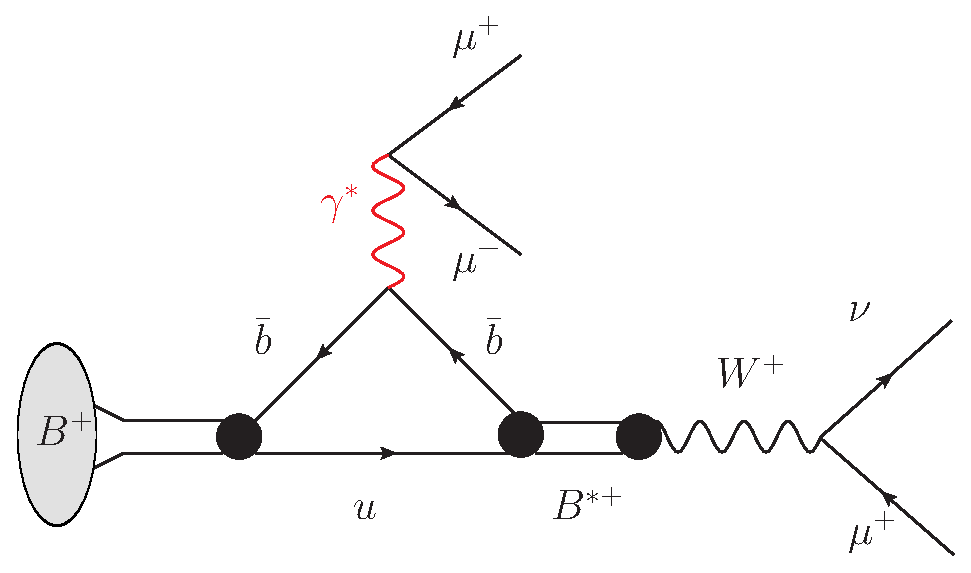
\includegraphics[width=0.45\linewidth]{Figure_1A.eps}
	  \hspace*{1.0cm}
    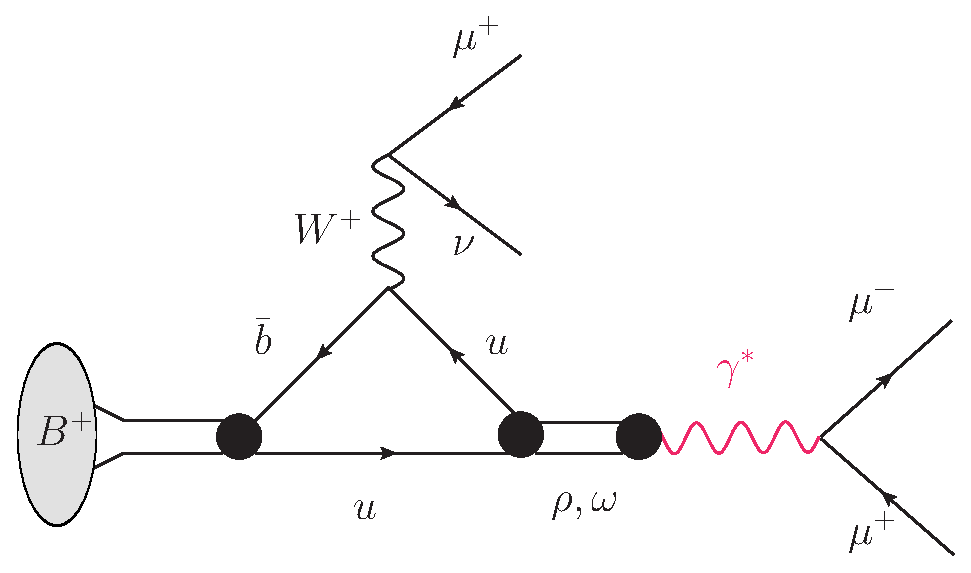
\includegraphics[width=0.45\linewidth]{Figure_1B.eps}
    \vspace*{-0.5cm}
  \end{center}
  \caption{Feynman diagrams of the dominant contributions (left)
    $\Bp\to\mup\neum\gamma^{*}$ with $\gamma^{*}\to\mumu$ and (right)
    $\Bp\to\mup\neum V$ to the \Bmumumu decay.}
  \label{fig:feyn}
\end{figure}

This paper describes a search for the decay \Bmumumu using a partial
reconstruction method that infers the momentum of the missing neutrino to
obtain a mass 
estimate of \Bmumumu decays. This search uses proton-proton ($pp$) collision
data corresponding to an integrated luminosity of $4.7\invfb$ collected during the  three periods 2011~(7\tev collision energy), 2012~(8\tev) and 2016~(13\tev)
at the LHCb experiment. The detector is described in Sec.~\ref{sec:Detector}, followed by a description of how
the signal is separated from backgrounds using two multivariate classifiers in Sec.~\ref{sec:Selection}. The
evaluation of the background is covered in Sec.~\ref{sec:Misid}, the normalisation of the branching fraction of
the signal to the decay $\decay{\Bp}{\jpsi \Kp}$ with $\decay{\jpsi}{\mup\mun}$ in Sec.~\ref{sec:Normalisation},
the limit on the branching fraction in Sec.~\ref{sec:results} and the systematic uncertainties in
Sec.~\ref{sec:systematics}. Finally, conclusions are presented in Sec.~\ref{sec:conclusions}.
